\documentclass[11pt,oneside]{report}

\usepackage[margin=0.9in,headheight=24pt]{geometry}
\usepackage[T1]{fontenc}
\usepackage[utf8]{inputenc}
\usepackage{amsmath,amssymb}
\usepackage{booktabs}
\usepackage{longtable}
\usepackage{array}
\usepackage{xcolor}
\usepackage{tikz}
\usepackage{hyperref}
\usepackage{enumitem}
\usepackage{listings}
\usepackage{titlesec}
\usepackage{fancyhdr}
\usepackage[protrusion=true,expansion=false]{microtype}

\usetikzlibrary{arrows.meta,calc,decorations.pathmorphing,positioning}

\definecolor{Ink}{HTML}{1B2430}
\definecolor{Muted}{HTML}{5B6472}
\definecolor{Accent}{HTML}{0077B6}
\definecolor{AccentTwo}{HTML}{D95F02}
\definecolor{Soft}{HTML}{F5F7FA}
\definecolor{SoftBlue}{HTML}{EAF4FB}
\definecolor{SoftOrange}{HTML}{FFF2E8}

\renewcommand{\familydefault}{\sfdefault}
\setlength{\parindent}{0pt}
\setlength{\parskip}{6pt}
\setlist{itemsep=2pt,topsep=4pt}

\hypersetup{
  colorlinks=true,
  linkcolor=Accent,
  urlcolor=Accent,
  citecolor=Accent
}

\lstdefinestyle{codestyle}{
  basicstyle=\ttfamily\small,
  backgroundcolor=\color{Soft},
  columns=fullflexible,
  keepspaces=true,
  breaklines=true,
  frame=leftline,
  framerule=2pt,
  rulecolor=\color{Accent},
  xleftmargin=0.8em,
  framesep=0.6em,
  showstringspaces=false
}
\lstset{style=codestyle}

\newcommand{\code}[1]{\texttt{#1}}
\newcommand{\ii}{\mathrm{i}}
\newcolumntype{L}[1]{>{\raggedright\arraybackslash}p{#1}}
\newcommand{\scopebox}[2]{%
  \par\smallskip
  \noindent\fcolorbox{#1!55!black}{#1!10}{%
    \begin{minipage}{0.96\linewidth}
    #2
    \end{minipage}}
  \par\smallskip
}
% Shared NMRSpinDynamics logo for LaTeX manuals.
% Expects the manuals' color palette and tikz package to be loaded.
\newcommand{\NMRSpinDynamicsLogo}[1][1]{%
  \begin{tikzpicture}[x=1cm,y=1cm,scale=#1,every node/.style={transform shape}]
    \fill[Soft] (0,0) rectangle (15.2,3.8);
    \draw[Accent!16,rounded corners=0.34cm,line width=0.7pt] (0,0) rectangle (15.2,3.8);

    \begin{scope}[shift={(1.75,1.9)}]
      \fill[white] (0,0) circle (1.22);
      \draw[Ink!13,line width=3.2pt] (0,0) circle (1.02);
      \draw[Accent,line width=4.4pt,line cap=round,rotate=-24]
        (0,0) ellipse (1.16 and 0.54);
      \draw[AccentTwo,line width=2.3pt,line cap=round,rotate=-24,opacity=0.58]
        (0,0) ellipse (1.16 and 0.54);
      \draw[Accent,line width=1.7pt,line cap=round,rotate=28,opacity=0.42]
        (0,0) ellipse (1.15 and 0.48);
      \draw[Ink,line width=4pt,line cap=round] (0,0) -- (0.78,0.69);
      \draw[Accent!85!green,line width=3.2pt,line cap=round] (0,0) -- (-0.45,-0.70);
      \fill[Ink] (0,0) circle (0.14);
      \fill[AccentTwo] (0.84,0.76) circle (0.14);
      \draw[AccentTwo,line width=2.3pt,line cap=round]
        (-1.02,-0.90) .. controls (-0.70,-0.60) and (-0.46,-0.60) .. (-0.14,-0.90)
        .. controls (0.18,-1.20) and (0.44,-1.20) .. (0.76,-0.90);
      \fill[Accent,rounded corners=0.05cm] (-1.13,0.15) rectangle (-1.00,0.95);
      \fill[Accent!85!green,rounded corners=0.05cm] (-0.85,0.00) rectangle (-0.72,1.12);
      \fill[AccentTwo,rounded corners=0.05cm] (-0.57,0.25) rectangle (-0.44,0.85);
    \end{scope}

    \node[anchor=west,inner sep=0pt,text=Ink,font=\sffamily\bfseries\fontsize{30}{34}\selectfont]
      at (3.65,2.25) {NMRSpinDynamics};
    \node[anchor=west,inner sep=0pt,text=Muted,font=\sffamily\fontsize{12}{14}\selectfont]
      at (3.70,1.56) {spin-1/2 simulations in inhomogeneous fields};
    \draw[Accent,line width=2.5pt,line cap=round] (3.72,0.92) -- (5.10,0.92);
    \draw[Accent!85!green,line width=2.5pt,line cap=round] (5.40,0.92) -- (6.78,0.92);
    \draw[AccentTwo,line width=2.5pt,line cap=round] (7.08,0.92) -- (8.46,0.92);
    \node[anchor=west,inner sep=0pt,text=Muted,font=\sffamily\fontsize{8}{10}\selectfont]
      at (3.72,0.43) {MATLAB reference and Python port};
  \end{tikzpicture}%
}


\titleformat{\chapter}[block]
  {\huge\bfseries\color{Ink}}
  {\color{Accent}\thechapter}
  {0.75em}
  {}
\titlespacing*{\chapter}{0pt}{-0.15in}{1.1em}
\titleformat{\section}
  {\Large\bfseries\color{Ink}}
  {\thesection}
  {0.6em}
  {}
\titleformat{\subsection}
  {\large\bfseries\color{Ink}}
  {\thesubsection}
  {0.6em}
  {}

\pagestyle{fancy}
\fancyhf{}
\lhead{\textcolor{Muted}{MATLABSpinDynamics}}
\rhead{\textcolor{Muted}{User Manual}}
\cfoot{\textcolor{Muted}{\thepage}}
\renewcommand{\headrulewidth}{0.3pt}
\renewcommand{\headrule}{\hbox to\headwidth{\color{Accent!35}\leaders\hrule height \headrulewidth\hfill}}

\begin{document}
\pagenumbering{gobble}
\begin{titlepage}
\pagecolor{Soft}
\color{Ink}
\vspace*{0.55in}
\begin{center}
\MRSpinDynamicsLogo[0.85]
\end{center}
\vspace{0.45in}
{\Huge\bfseries MATLABSpinDynamics\par}
\vspace{0.25in}
{\Large User Manual\par}
\vspace{0.15in}
{\large Reference MATLAB implementation for NMR spin-dynamics simulations\par}
\vspace{0.45in}
{\color{Accent}\rule{0.82\linewidth}{3pt}\par}
\vspace{0.35in}
\begin{minipage}{0.78\linewidth}
\large
Classical isochromat simulations for uncoupled spin-1/2 nuclei in
non-uniform and time-varying magnetic fields, with ideal, tuned, untuned,
and impedance-matched probe workflows.
\end{minipage}
\vfill
{\large June 2026\par}
\end{titlepage}
\nopagecolor
\clearpage
\pagenumbering{roman}
\tableofcontents
\clearpage
\pagenumbering{arabic}

\chapter{Physical Scope and Assumptions}

MATLABSpinDynamics models a bath of uncoupled spin-1/2 nuclei in a main field
\(B_0(\mathbf{r},t)\) that may be non-uniform, time-varying, or both. The
sample is discretized into isochromats. Each isochromat represents a small
subensemble that shares an offset, RF sensitivity, relaxation constants, and
probe response.

\scopebox{Accent}{
\textbf{Modeled directly.} Independent spin-1/2 magnetization vectors; offset
distributions from \(B_0(\mathbf{r},t)\); RF rotations; free precession;
phenomenological relaxation; diffusion in selected workflows; phase encoding;
and probe-circuit transmit/receive filtering.
}

\scopebox{AccentTwo}{
\textbf{Not modeled explicitly.} Spin-spin coupling, J-coupling networks,
dipolar coupling, spins with \(I>1/2\), quadrupolar transitions,
multi-quantum coherences, density-matrix entanglement, chemical exchange, and
microscopic spin noise. These effects only enter indirectly if represented by
effective relaxation constants, diffusion terms, or supplied field maps.
}

This is a Bloch/isochromat simulator, not a general quantum spin Hamiltonian
solver. It is most useful when the experiment can be described by the motion of
classical magnetization vectors under prescribed fields and circuit response.

\section{Spin Bath Cartoon}

\begin{center}
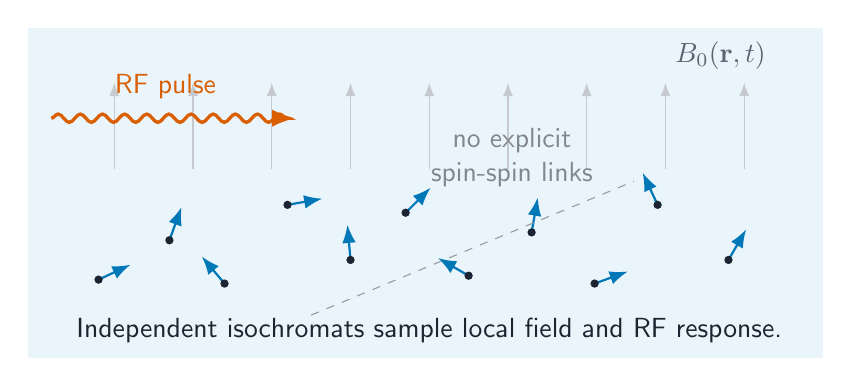
\begin{tikzpicture}[x=1cm,y=1cm,>=Latex]
  \fill[SoftBlue] (-0.4,-0.4) rectangle (9.7,3.8);
  \foreach \x/\y/\a in {
    0.5/0.6/25, 1.4/1.1/70, 2.1/0.55/130, 2.9/1.55/10,
    3.7/0.85/95, 4.4/1.45/45, 5.2/0.65/150, 6.0/1.2/80,
    6.8/0.55/20, 7.6/1.55/115, 8.5/0.85/60}
  {
    \draw[Accent,thick,->] (\x,\y) -- ++(\a:0.45);
    \fill[Ink] (\x,\y) circle (1.5pt);
  }
  \foreach \x in {0.7,1.7,...,8.7}
  {
    \draw[Muted!35,->] (\x,2.0) -- ++(0,1.1);
  }
  \node[Muted] at (8.4,3.45) {$B_0(\mathbf{r},t)$};
  \draw[AccentTwo,very thick,decorate,decoration={snake,amplitude=1.5pt,segment length=8pt},->]
    (-0.1,2.65) -- (3.0,2.65);
  \node[AccentTwo] at (1.35,3.05) {RF pulse};
  \draw[Ink!45,dashed] (3.2,0.15) -- (7.3,1.85);
  \node[Ink!55,align=center] at (5.75,2.15) {no explicit\\spin-spin links};
  \node[align=left,Ink] at (4.7,-0.05) {Independent isochromats sample local field and RF response.};
\end{tikzpicture}
\end{center}

\section{Practical Consequences}

\begin{itemize}
  \item Use offset grids or field maps to represent \(B_0\) inhomogeneity.
  \item Use transmit and receive \(B_1\) maps or probe models to represent RF
  non-uniformity and circuit filtering.
  \item Use \(T_1\), \(T_2\), diffusion, or effective field maps to capture
  physics outside the explicit uncoupled-spin model.
  \item Avoid using this code for phenomena that require explicit coupled-spin
  quantum pathways.
\end{itemize}

\chapter{Installation Requirements}

\section{MATLAB Path Setup}

No packaging step is required. From the \code{MATLABSpinDynamics} directory,
add the active Version 3 code tree to the MATLAB path:

\begin{lstlisting}
repo = pwd;
addpath(genpath(fullfile(repo, 'Version_3', 'code')));
\end{lstlisting}

For a script launched elsewhere, replace \code{pwd} with the absolute path to
\code{MATLABSpinDynamics}. The exact minimum MATLAB release has not been pinned.
Use a recent MATLAB release for the current Version 3 scripts and graphics.

\section{GNU Octave Compatibility}

Most core numerical functions and base examples are compatible with GNU Octave.
The Python port's parity fixtures were largely generated from MATLAB/Octave
reference scripts, and a compact Octave smoke check against \code{Version\_3/code}
currently covers representative echo, parameter-constructor, and ideal
asymptotic-magnetization routines.

Octave compatibility is not universal. Workflows that use \code{fmincon},
\code{optimoptions}, MATLAB Coder/MEX generation, \code{parfor}, or MATLAB-only
graphics/toolbox behavior still require MATLAB or local script edits. In a
stock Octave install, optimization workflows are the main gap.

\section{Core and Optional Dependencies}

\begin{longtable}{L{0.31\linewidth}L{0.58\linewidth}}
\toprule
Requirement & When it is needed \\
\midrule
Base MATLAB & Core ideal spin dynamics, many low-level rotation/echo helpers,
and many basic probe examples. \\
Parallel Computing Toolbox & Workflows that use \code{parfor}, including many
Q sweeps, mistuning sweeps, imaging scripts, CPMG-IR scripts, and optimization
repeats. Convert \code{parfor} to \code{for} for smaller serial runs. \\
Optimization Toolbox & Matched-probe network design and pulse optimization
workflows using \code{fmincon} or \code{optimoptions}. \\
Image Processing Toolbox & Imaging examples that call \code{imresize} or
\code{rgb2gray}. \\
MATLAB Coder and C/C++ compiler & Optional MEX/code-generation build scripts
under \code{Version\_3/code/mex}. Configure the compiler
with \code{mex -setup}. Generated MEX/codegen outputs are local build artifacts
and are ignored by Git. \\
\code{export\_fig} & Optional third-party File Exchange helper used by some
plotting/export scripts through \code{safe\_export\_fig}. Missing
\code{export\_fig} causes exports to be skipped with a warning. \\
\bottomrule
\end{longtable}

Use \code{ver} in MATLAB to inspect installed toolboxes before running a
workflow. Missing optional toolboxes do not prevent the base simulation
functions from being used.

\chapter{Repository Map}

\begin{longtable}{L{0.36\linewidth}L{0.56\linewidth}}
\toprule
Path & Purpose \\
\midrule
\path{Version_3/code} & Recommended active MATLAB code. \\
\path{Version_2} & Earlier updated implementation kept for
historical comparison. \\
\path{Version_1} & Legacy original implementation. \\
\path{docs/QUICK_START.md} & Practical starting guide for common MATLAB runs. \\
\path{docs/VERSION_GUIDE.md} & Map of active, legacy, and repeated functions. \\
\path{docs/VERSION_3_WORKFLOWS.md} & Workflow-oriented guide to Version 3 scripts. \\
\path{docs/SPEED_AUDIT.md} & Performance observations and acceleration notes. \\
\bottomrule
\end{longtable}

\chapter{Model Conventions}

\section{Isochromat Evolution}

The simulation discretizes the sample into offsets \(\Delta\omega_k\) and, when
needed, transmit/receive sensitivities. For a rectangular RF interval with
amplitude \(\omega_1\), phase \(\phi\), and duration \(t\), the rotating-frame
effective field is
\[
  \boldsymbol{\Omega}_k =
  \begin{bmatrix}
    \omega_1 \cos\phi \\
    \omega_1 \sin\phi \\
    \Delta\omega_k
  \end{bmatrix},
  \qquad
  \Omega_k = \|\boldsymbol{\Omega}_k\|.
\]
The magnetization update is a rotation by \(\Omega_k t\) about
\(\boldsymbol{\Omega}_k/\Omega_k\). The axis and angle generally differ across
isochromats because offsets and RF sensitivities differ.

\section{Normalized Time}

The bare spin-dynamics functions use normalized units with \(\omega_1=1\).
Thus a nominal 90-degree pulse has duration
\[
  t_{90} = \frac{\pi}{2},
\]
and a nominal 180-degree pulse has duration
\[
  t_{180} = \pi .
\]
Probe-aware workflows often use physical seconds internally or in their
parameter structures. When mixing bare and probe-aware code, check whether each
function expects normalized or physical time.

\section{Pulse Timing Cartoon}

\begin{center}
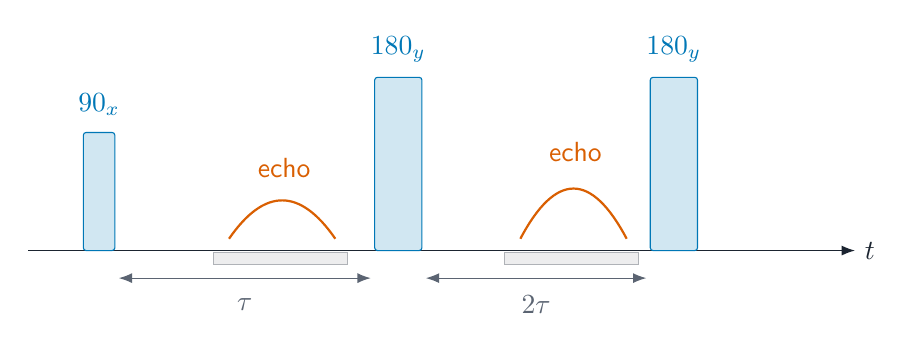
\begin{tikzpicture}[x=1cm,y=1cm,>=Latex]
  \draw[Ink,->] (0,0) -- (10.5,0) node[right] {$t$};
  \draw[Accent,fill=Accent!18,rounded corners=1pt] (0.7,0) rectangle (1.1,1.5);
  \node[Accent] at (0.9,1.85) {$90_x$};
  \draw[Accent,fill=Accent!18,rounded corners=1pt] (4.4,0) rectangle (5.0,2.2);
  \node[Accent] at (4.7,2.55) {$180_y$};
  \draw[Accent,fill=Accent!18,rounded corners=1pt] (7.9,0) rectangle (8.5,2.2);
  \node[Accent] at (8.2,2.55) {$180_y$};
  \draw[Muted,<->] (1.15,-0.35) -- (4.35,-0.35);
  \node[Muted] at (2.75,-0.68) {$\tau$};
  \draw[Muted,<->] (5.05,-0.35) -- (7.85,-0.35);
  \node[Muted] at (6.45,-0.68) {$2\tau$};
  \draw[AccentTwo,thick] (2.55,0.15) .. controls (3.0,0.8) and (3.45,0.8) .. (3.9,0.15);
  \node[AccentTwo] at (3.25,1.05) {echo};
  \draw[AccentTwo,thick] (6.25,0.15) .. controls (6.7,1.0) and (7.15,1.0) .. (7.6,0.15);
  \node[AccentTwo] at (6.95,1.25) {echo};
  \draw[Ink!35,fill=Ink!8] (2.35,-0.02) rectangle (4.05,-0.18);
  \draw[Ink!35,fill=Ink!8] (6.05,-0.02) rectangle (7.75,-0.18);
\end{tikzpicture}
\end{center}

\section{Rotation Cartoon}

\begin{center}
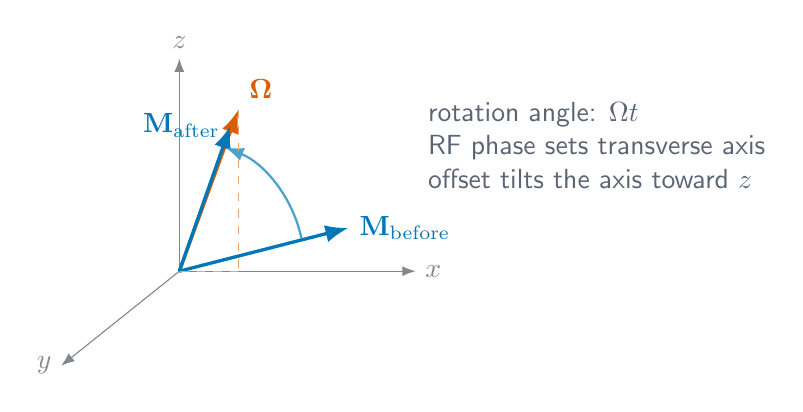
\begin{tikzpicture}[x=1cm,y=1cm,>=Latex]
  \coordinate (O) at (0,0);
  \draw[Ink!55,->] (O) -- (3.0,0) node[right] {$x$};
  \draw[Ink!55,->] (O) -- (0,2.7) node[above] {$z$};
  \draw[Ink!55,->] (O) -- (-1.5,-1.2) node[left] {$y$};
  \draw[AccentTwo,very thick,->] (O) -- (0.75,2.05) node[above right] {$\boldsymbol{\Omega}$};
  \draw[Accent,very thick,->] (O) -- (2.15,0.55) node[right] {$\mathbf{M}_{\mathrm{before}}$};
  \draw[Accent,very thick,->] (O) -- (0.65,1.85) node[left] {$\mathbf{M}_{\mathrm{after}}$};
  \draw[Accent!70,thick,->] (1.55,0.42) arc[start angle=12,end angle=68,radius=1.6];
  \node[Muted,align=left] at (5.3,1.6) {
    rotation angle: $\Omega t$\\
    RF phase sets transverse axis\\
    offset tilts the axis toward $z$
  };
  \draw[AccentTwo!55,dashed] (0.75,2.05) -- (0.75,0);
  \draw[AccentTwo!55,dashed] (0.75,0) -- (0,0);
\end{tikzpicture}
\end{center}

\section{Relaxation and Diffusion}

Default bare functions omit relaxation and diffusion for speed. Relaxation
variants apply exponential updates such as
\[
  M_{xy}(t+\Delta t) =
    M_{xy}(t)\exp\left(-\frac{\Delta t}{T_2}\right)
    \exp(-\ii \Delta\omega\,\Delta t),
\]
\[
  M_z(t+\Delta t) =
    M_{\mathrm{eq}} +
    \left(M_z(t)-M_{\mathrm{eq}}\right)
    \exp\left(-\frac{\Delta t}{T_1}\right).
\]
Diffusion-aware workflows add attenuation or state updates specific to the
selected pulse sequence and probe model.

\chapter{First Workflow}

\section{A Minimal Ideal CPMG Calculation}

The lower-level MATLAB interface builds pulse intervals and passes them to
rotation/echo helpers. A stripped-down CPMG calculation looks like this:

\begin{lstlisting}
numpts = 2001;
maxoffs = 20;
del_w = linspace(-maxoffs, maxoffs, numpts);

tacq = 5*pi;
window = sinc(del_w*tacq/(2*pi));
window = window ./ sum(window);

texc = [pi/2 -1];
pexc = [pi/2 0];
aexc = [1 0];

tref = pi*[3 1 3];
pref = [0 0 0];
aref = [0 1 0];

neff = calc_rot_axis_arba3(tref, pref, aref, del_w, 0);
masy1 = sim_spin_dynamics_asymp_mag3(texc, pexc, aexc, neff, del_w, tacq);
masy2 = sim_spin_dynamics_asymp_mag3(texc, pexc + pi, aexc, neff, del_w, tacq);
masy = (masy1 - masy2)/2;

snr = trapz(del_w, abs(masy).^2);
[echo, tvect] = calc_time_domain_echo(masy, del_w);
\end{lstlisting}

Many production scripts use \code{set\_params\_*} helpers instead of spelling
out every interval by hand. Those helpers create MATLAB structures, usually
named \code{sp}, \code{pp}, and sometimes \code{params}, that carry simulation,
pulse, and circuit settings.

\section{Probe-Aware Workflows}

Probe-aware scripts model untuned, tuned, and impedance-matched probes. The
main caution is unit conversion: bare spin-dynamics routines commonly expect
normalized time, while circuit workflows may use physical seconds and convert
internally. Always check the function help and nearby workflow script before
mixing pieces from different folders.

\chapter{Workflow Map}

\begin{longtable}{L{0.32\linewidth}L{0.58\linewidth}}
\toprule
Folder or family & Typical use \\
\midrule
\code{calc\_rot} & Effective rotation axes, rotation matrices, critical
offsets, and probe-aware pulse response helpers. \\
\code{calc\_echo} & Frequency-domain to time-domain echo conversion. \\
\code{sim\_spin\_dynamics\_asymp} & Asymptotic and excitation spin-dynamics
kernels for ideal CPMG-style studies. \\
\code{cpmg\_*} and probe folders & Ideal, tuned, untuned, and matched CPMG
sequence calculations. \\
\code{CompareQ} & Quality-factor sweeps for tuned and matched probes. \\
\code{CompareMistuned} & Probe mistuning studies. \\
\code{CPMG\_IR} & CPMG inversion-recovery workflows. \\
\code{Images} and imaging scripts & Phase-encoded imaging examples and
field-map helpers. \\
\code{Sim\_Diffusion} and \code{calc\_macq\_diff} & Diffusion-aware matched
probe spin-echo and CPMG variants. \\
\code{time\_varying\_field} & CPMG under prescribed time-varying fields. \\
\code{Wurst\_Inversion} & WURST inversion and matched WURST-CPMG studies. \\
\code{opt\_pulse} & Refocusing and excitation pulse optimization. \\
\code{mex} & Optional compiled-kernel/code-generation experiments. \\
\bottomrule
\end{longtable}

\chapter{Function Family Reference}

\section{Bare Spin Dynamics}

Start here when developing or validating a new pulse sequence:

\begin{lstlisting}
calc_rotation_matrix
calc_rot_axis_arba3
calc_rot_axis_arba4
sim_spin_dynamics_asymp_mag3
sim_spin_dynamics_exc
calc_time_domain_echo
calc_time_domain_echo_arb
\end{lstlisting}

These functions expose the core interval representation: durations, RF phases,
RF amplitudes, offsets, and acquisition flags. They are fast and close to the
underlying Bloch/isochromat model, but they leave more setup work to the user.

\section{Parameter Constructors}

Many workflow scripts use \code{set\_params\_*} functions to assemble default
simulation and pulse structures:

\begin{lstlisting}
set_params_ideal
set_params_tuned_orig
set_params_untuned_orig
set_params_matched_orig
set_params_tuned_spa
set_params_untuned_spa
set_params_matched_spa
set_params_matched_SS
\end{lstlisting}

Treat these functions as executable documentation. They are often the clearest
place to find default pulse lengths, acquisition windows, Q values, matching
network values, and relaxation settings.

\section{Probe Models}

\begin{lstlisting}
tuned_probe_lp
tuned_probe_rx
tuned_probe_rx_tf
untuned_probe_lp
untuned_probe_rx
untuned_probe_rx_tf
matching_network_design2
find_coil_current
find_coil_current_WURST
matched_probe_rx
\end{lstlisting}

The tuned and untuned helpers model transmit/receive filtering directly. The
matched-probe path includes circuit design and coil-current calculations, and
therefore may require Optimization Toolbox for design-time routines.

\section{Pulse Shapes and Optimization}

\begin{lstlisting}
create_WURST
quantize_phase
untuned_pulse_adjust
opt_ref_pulse_tuned
opt_ref_pulse_untuned
opt_ref_pulse_matched
opt_exc_pulse_tuned
\end{lstlisting}

Optimization scripts often use \code{parfor} for repeated random starts and
\code{fmincon} for local constrained optimization. For quick experiments,
reduce the number of starts or replace \code{parfor} loops with ordinary
\code{for} loops.

\section{Generated or Compiled Kernels}

The \code{mex} folder contains optional build scripts for compiled kernels.
These are not required for ordinary use. Generated MEX files and codegen
reports are ignored release artifacts. Rebuild them locally with MATLAB Coder
and a configured compiler:

\begin{lstlisting}
mex -setup
\end{lstlisting}

\chapter{Validation and Porting Notes}

The sibling Python package uses this MATLAB Version 3 tree as its numerical
reference. When changing MATLAB behavior, update the relevant fixture scripts
and document whether the Python port should follow the new behavior or preserve
older compatibility.

Good validation practice is:

\begin{itemize}
  \item create a small MATLAB script that exercises the exact function family;
  \item save compact arrays rather than large figures or workspace dumps;
  \item test ideal kernels before adding probe response, relaxation, diffusion,
  or optimization;
  \item record unit conventions, especially normalized time versus seconds.
\end{itemize}

\chapter{Known Caveats}

This repository contains multiple generations of related functions. Names are
sometimes repeated across folders. Prefer the active Version 3 code tree for new
work, check \code{docs/VERSION\_GUIDE.md} when a function appears in more than
one place, and keep local path edits out of numerical changes.

The code is strongest as a research reference and simulation toolkit. It is not
currently packaged as a MATLAB Toolbox app, and it does not try to hide every
experimental script behind a single stable API.

\end{document}
